\documentclass[11pt]{article}
\usepackage[utf8]{inputenc}
\usepackage{amsmath}
\usepackage[margin=1in]{geometry}
\usepackage{xcolor}
\usepackage{graphicx}

\begin{document}

\newcommand{\Dfrac}[2]{%
  %\left(
  \ooalign{%
    $\genfrac{}{}{1.2pt}0{#1}{#2}$\cr%
    $\color{white}\genfrac{}{}{.4pt}0{\phantom{#1}}{\phantom{#2}}$}%
  %\right)
}
\newcommand{\cond}{\middle\vert}



\begin{center}
\begin{tabular}{lll}
Symbol & Time & Meaning\\
\hline
$p$ & $t-1$ & Parental generation\\
$c$ & $t-\frac{1}{2}$ & Contributing (intermediate, selection only)\\
$o$ & $t$ & Offspring (current) generation\\
\end{tabular}
\end{center}



\begin{center}
\begin{tabular}{ll}
Symbol & Meaning\\
\hline
$n$ & Sample size\\
$i$ & Number of derived alleles in sample $n_{\cdot}$\\
$\Dfrac{i}{n}$ & $i$ derived \emph{out of} $n$ alleles\\
\end{tabular}
\end{center}


\section{Background}

We want to describe the behavior of $n$ biallelic loci from a Wright-Fisher model with population
size $N$. Specifically, we seek an expression for the transition probability matrix $\mathbf{P}$ for
the time evolution of the \emph{AFS}, $\Phi$:

\begin{equation}
  \label{eq:app:time-evolution}
  \Phi_n^{(t)} = \mathbf{P}_n \Phi_n^{(t-1)}
\end{equation}

$\mathbf{P}_n$ is a square $n \times n$ matrix, and it enumerates the number of derived alleles ($i$) at a
biallelic locus in a sample of size $n$. We will need to keep track of these quantities in the
offspring ($o$), parents ($p$), and contributing ($c$) lineages for a given generation (table X).
For example, $\Dfrac{i_p}{n_p}$ (read as "$i_p$ out of $n_p$") denotes a sample of size $n$ with $i$
derived in the parental generation (time $t-1$).

Instead of using the summation formulation presented in the main text \eqref{eq:ZZ}, we use
recursive conditional probabilities, where the transitions are defined in terms of transitions in
smaller sample sizes. Each entry of the matrix, $\mathbf{P}_{(i_o,i_p)}$ is a conditional transition
probability. The key observation is that we can condition on a set of coalescent events,
$\{\Lambda\}$:

\begin{align*}
  P\left[\Dfrac{i_o}{n_o} \cond \Dfrac{i_p}{n_p}\right] &= \sum_{\lambda\in\{\Lambda\}}P(\lambda)
  P\left[\Dfrac{i_o}{n_o} \cond \Dfrac{i_p}{n_p},\lambda\right] \\
  &= \sum_{\lambda\in\{\Lambda\}}P(\lambda)
  P\left[\Dfrac{i_o-|\lambda|_{i_o}}{n_o-|\lambda|_{n_o}} \cond \Dfrac{i_p-|\lambda|_{i_p}}{n_p-|\lambda|_{n_p}}\right]
\end{align*}

Above, $|\lambda|$ denotes the size of the coalescent event. The second equation ascertains that
conditioning on a coalescent event is equivalent to subtracting relevant lineages from the sample.
This gives rise to a recurrence, where transition probabilities in a sample of size $n$ can be
described recursively in terms of transition probabilities in smaller sample sizes, $n' \in [1, n-1]$.

\section{Neutral case}


Under neutrality, the number of parental lineages that contribute to the current generation can not
be larger than the offspring sample size. Thus we can condition on the parental configuration
directly, seeking $P\left[\Dfrac{\cdot}{n_o} \cond \Dfrac{\cdot}{n_p}\right]$. This probability can be
constructed recursively in terms of $P\left[\Dfrac{i_o}{n_o-1} \cond \Dfrac{i_p}{n_p}\right]$

The second equation follows since conditioning on a coalescent event is equivalent to decreasing the
size 

Instead of using the summation formulation presented in the main text, we seek a recursive
construction of $Q_n$ in terms of transition probability matrices $Q_{n'}$, $n' \in [1, n-1]$. This
approach simplifies accounting for multiple coalescent events per generation, and is amenable to a
dynamic programming implementation.

The transition probability matrix enumerates the number of derived alleles ($i$) at a biallelic
locus in a sample of size $n$. We will need to keep track of these quantities in the offspring
($o$), parents ($p$), and gametes ($g$) for a given generation (table X). We denote the
configuration as a tuple - for example the present (offspring) generation, $(i_o, n_o)$.

We want to construct conditional transition probabilities of the form $P[(i_o,n_o)|(i_p,n_p)]$ in
terms of probabilities for smaller sample sizes: $P[(i_o',n_o-1)\mid(i_p',n_p-1)]$. This can be done if
condition on coalescent events $\Lambda$ for sample size $n$

\begin{equation}
P[(i_o,n_o)\mid(i_p,n_p)] = \sum_{a=\{der,anc\}}f_a\sum_{\Lambda}P(\Lambda) P[(i_o,n_o)\mid(i_p,n_p),\Lambda]
\end{equation}

Conditioning on the coalescent event will decrease the number of available alleles in both parental
and offspring generation. For example, conditioning on a coalescent event that includes an ancestral
allele will decrease the total number of lineages, while keeping the number of derived lineages constant.


\section{Neutral case}


We want to construct the entries in the probability matrix $P\left[ \Dfrac{\cdot}{n_o} \cond
  \Dfrac{\cdot}{n_p} \right]$ in terms transition probabilities in smaller sample sizes. Under
neutrality, the number of contributing parental lineages $n'_p$ (at $t-1$) can not be larger than
the number of offspring lineages $n_o$. Since $\mathbf{P}$ is square, $max(n_p)=max(n_o)=n$. Thus,
our aim is to express every entry of $\mathbf{P}$, $P\left[ \Dfrac{\cdot}{n} \cond\Dfrac{\cdot}{n}
  \right]$, in terms of $P\left[ \Dfrac{\cdot}{n-1} \cond \Dfrac{\cdot}{n-1} \right]$.


To do so, we first condition on the state of the last parental allele drawn, and then on the
coalescent event that last offspring lineage participates in. The recurrence is shown in equation \eqref{}

 We condition on the state of the last parental allele drawn,
and on the parental lineage drawn for the last offspring.

\begin{equation}
  \begin{aligned}
    P\left[ \Dfrac{i_o}{n_o} \cond \Dfrac{i_p}{n_p} \right] = \left( \frac{n-i_o}{n} \right) 
    & \Bigg\{ \left( 1-\frac{n-1}{N}   \right)  P \left[ \Dfrac{i_o}{n_o-1}   \cond \Dfrac{i_p}{n_p-1} \right] \\
    & +       \left( \frac{i_o}{N} \right)      P \left[ \Dfrac{i_o-1}{n_o-1} \cond \Dfrac{i_p}{n_p-1} \right] \\
    & +       \left( \frac{n-i_o-1}{N} \right)  P \left[ \Dfrac{i_o}{n_o-1}   \cond \Dfrac{i_p}{n_p-1} \right] \Bigg\} \\
    \left( \frac{i_o}{n_o} \right) 
    & \Bigg\{  \left( 1 - \frac{n-1}{N} \right) P \left[ \Dfrac{i_o-1}{n_o-1} \cond \Dfrac{i_p-1}{n_p-1} \right] \\
    & +       \left( \frac{i_o-1}{N} \right)    P \left[ \Dfrac{i_o-1}{n_o-1} \cond \Dfrac{i_p-1}{ n_p-1} \right] \\
    & +       \left( \frac{n-i_o}{N} \right)    P \left[ \Dfrac{i_o}{n_o-1}   \cond \Dfrac{i_p-1}{n_p-1} \right] \Bigg\}
  \end{aligned}
\end{equation}

The base cases of the rucurrence happen with $n=1$:
\begin{align*}
  P\left[ \Dfrac{1}{1} \cond \Dfrac{1}{1} \right] &= 1 \\
  P\left[ \Dfrac{0}{1} \cond \Dfrac{0}{1} \right] &= 1 \\
  P\left[ \Dfrac{0}{1} \cond \Dfrac{1}{1} \right] &= 0 \\
  P\left[ \Dfrac{1}{1} \cond \Dfrac{0}{1} \right] &= 0 \\
\end{align*}

\begin{figure}[ht]
  \centering
  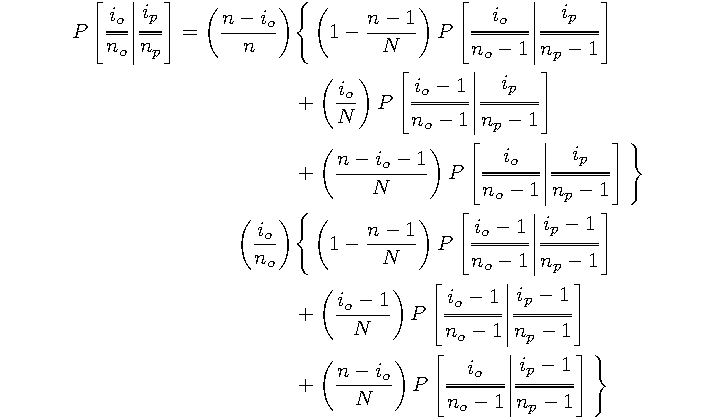
\includegraphics[width=0.5\textwidth]{fig/recurrence-neutral.pdf}
  \caption{Schematic version of equation XX}
\end{figure}



\section{Selection case}

Due to selective deaths, the number of lineages that contribute to offspring ($n_c$) can be
significantly larger than the number of offspring ($n_o$) with strong selection. We use $n_c$, the
intermediate number of lineages at time $t-\frac{1}{2}$, which can potentially be much larger than
the number of parents, $n_p$. This is analogous to the gamete intermediates, as presented in the
main text. However, the two are not equivalent, since in this formulation we apply selection
\emph{and} drift on the intermediate lineages.

\begin{equation}
  P\left[ \Dfrac{i_o}{n} \cond \Dfrac{i_p}{n} \right] = \sum_{i_c,n_c}P\left[ \Dfrac{i_o}{n}
    \cond \Dfrac{i_c}{n_c} \right] P\left[ \Dfrac{i_c}{n_c} \cond \Dfrac{i_p}{n} \right]
\end{equation}

\begin{aligned}
  n_p &= n \\
  i_p &\in [0, n] \\
  n_c &\in [1, n] \\
  i_c &\in [0, n_c] \\
\end{aligned}

The probability conditional on the contributing lineages is in equation XX, while $P\left[
  \Dfrac{i_c}{n_c} \cond \Dfrac{i_p}{n} \right]$ is given by the hypergeometric distribution. The
support of the hypergeometric distribution means that we can not have $n_c>n$. Note
that while $i_c \le n_c \le n$, we can still have $i_c>i_p$ if $i_p$ is small. A formulation where a
$n_c$ is potentially infinitely large will be desirable.

The recursive definition, analogous to equation XX provides $P\left[ \Dfrac{i_o}{n}
    \cond \Dfrac{i_c}{n_c} \right]$, the probability that $i_o$ out of $n$ lineages are derived, given
that $i_c$ out of $n_c$ contributed to it. To construct this probability, we condition on the
coalescent events involving the last offspring allele. There are 6 distinct coalescent events, with
distinct probabilities based on whether the last offspring allele is ancestral or derived. This
gives 12 different cases.

\end{document}
